\documentclass[11pt,a4paper]{scrartcl}
\typearea{12}
\usepackage{graphicx}
\usepackage{pstricks}
\usepackage{listings}
\lstset{language=python}
\pagestyle{headings}
\markright{Computation Neuroscience -  4 integrate and fire}
\begin{document}

\subsection*{Introduction}
This note is about the dynamics of a single neuron, it will cover
one of the simplest such models: the leaky integrate and fire model.

\subsection*{Electrical properties of a neuron}
The potential inside a neuron is lower than the potential on the
outside; this difference is created by ion pumps, small molecular
machines that use energy to pump ions across the membrane seperating
the inside and outside of the cell. One typical ion pump is
Na+/K+-ATPase (Sodium-potassium adenosine triphosphatase); this uses
energy in the form of ATP, the energy carrying molecule in the body,
and through each cycle it moves three sodium ions out of the cell and
two potassium ions into the cell. Since both sodium and potassium ions
have a charge of plus one, this leads to a net loss of one atomic
charge to the inside of the cell lowering its potential. It also
creates an excess of sodium outside the cell and an excess of
potassium inside it. We will return to these chemical imbalances
later. The potential difference across the membrane is called the
\textbf{membrane potential}. At rest a typical value of the membrane
potential is $E_L=-70 $mV. It is useful to remember that the excessive
sodium is outside the cell and potassium inside; I think of islands
which are surrounded by salty water.

\subsection*{Spikes}

So the summary version of what happens in neuons is that
\textbf{synapses} cause a small increase or decrease in the voltage;
\textbf{excitatory synapses} cause an increase, \textbf{inhibitory
  synapses} a decrease. This drives the internal voltage dynamics of
the cell, these dynamics are what we will learn about here. If the
voltage exceeds a threshold, say $V_T=-55$ mV there is a nonlinear
cascade which produces a \textbf{spike} or \textbf{action potential},
a spike in voltage 1-2 ms wide which rises above 0 mV before, in the
usual description, falling to a reset value of $V_R=-65$ mV, the cell
then remains unable to produce another spike for a \textbf{refractory
  period} which may last about 5 ms. We will examine how spikes are
formed later, this involves the nonlinear dynamics of ion channels in
the membrane; first though we will consider the integrate and fire
model which ignores the details of how spikes are produced and
simplifies the voltage dynamics.

\subsection*{The bucket-like equation for neurons}

We will now try to extend the bucket-like equation we looked at before
so that it applies to neurons. First off we replace $h$, the height of
the water, by $V$ the voltage in the cell and $C$ will be replaced by
$C_m$, the capacitance of the membrane, the amount of electrical
charge that can be stored at the membrane is $C_mV$. The amount of
electrical charge is the analogue of the volume of water. Thus,
voltage is like height, charge is like the amount of water.

The leak is a bit more complicated, because of the chemical gradients,
that is the effects of the differing levels of ions inside and outside
the cell along and their propensity to diffuse, the voltage at which
there is no leaking of charge is not zero, it is $E_L=-70 $mV,
roughly. This is an important aspect of how neurons behave, and one we
will encounter again looking at the Hodgkin-Huxley equation: you might
at first expect that if the voltage inside the cell was, say, -60 mV
then even if there was a high conductivity for potassium at the
membrane, the potassium ions would stay in the cell: they are positive
ions after all and so a negative voltage means the electrical force is
attracting them to the inside of the cell. However, this isn't quite
what happens, there is a high concentration of potassium inside the
cell and because of the random motion of particles associated with
temperature, these have a tendency to diffuse, that is to increase the
entropy of the situation by spreading out. It takes a force to
counteract this. This is the reversal potential, $E_L$, the voltage required
for zero current even if there is some conductivity.

$G$ is now $G_m$, a conductance, measuring the porousness of the
membrane to the flow of ions. The leak current is $G_m(V-E_L)$, as
above, we actually divide across by it, and write $R_m=1/G_m$, the
resistance. Finally, we write $\tau_m=C_m/G_m$ to get
\begin{equation}
\tau_m\frac{dV}{dt}=E_L-V+R_mI
\end{equation}
$I$ might end up being synaptic input, but traditionally we write the
equation to match the \textsl{in vivo} experiment where $I$ is an
injected current from an electrode, so we write $I_e$, \lq{}e\rq{} for
electrode. $tau_m$ is a time constant, using the notation of
dimensional analysis we have $[\tau_m]=T$. To check this note that the
units of capacitance are charge per voltage: $[C_m]=QV^{-1}$, the
units of resistance is voltage per current $[R_m]=VI^{1}$ and current
is charge per time, $[I]=QT^{-1}$ so $[C_mR_m]=T$, time.

The equation above leaves out the possibility that there are other
non-linear changes in the currents through the membrane as $V$
changes. This is a problem since there are other non-linear changes in
the currents through the membrane as $V$ changes. The equation above
leaves these out, in fact, the nonlinear effects are strongest for
values of $V$ near where a spike is produced, so one approach is to
use the linear equation unless $V$ reaches a threshold value and then
add a spike \lq{}by hand\rq{}. This has the effect of changing the
voltage to a reset value, this mimics what happens in the neuron, or
in the Hodgkin Huxley model which we will look at next and which
includes the full non-linear dynamics which makes the spike. Anyway,
in summary
\begin{itemize}
\item $V$ satisfies
\begin{equation}
\tau_m\frac{dV}{dt}=E_L-V+R_mI_e
\end{equation}
\item If $V\ge V_T$ a spike is recorded and the voltage is set to a
  reset value $V_R$.
\end{itemize}
The reset value, the voltage after the spike is often set equal to the
 leak potential. This is the \textbf{leaky integrate and fire model}, a surprisingly
old model first introduced in \cite{Lapicque1907a}. It lacks lots of
the details important in the dynamics of neurons, but is useful and
often used for modeling the behavior of large neuronal networks or for
exploring ideas about neuronal computation in a relatively
straight-forward setting.

This model is easy to solve; if $I_e$ is constant we have already
solved it above up to messing around with constants:
\begin{equation}
V(t)=E_L+R_mI_e+[V(0)-E_L-R_mI_e]e^{-t/\tau_m}
\end{equation}
If $I_e$ is not
constant it may still be possible to solve the equation, but in any
case the equation can be solved numerically on a computer. An example
in given in Fig.~\ref{v_i_f}.

\begin{figure}
\begin{center}
% GNUPLOT: LaTeX picture with Postscript
\begingroup
  \makeatletter
  \providecommand\color[2][]{%
    \GenericError{(gnuplot) \space\space\space\@spaces}{%
      Package color not loaded in conjunction with
      terminal option `colourtext'%
    }{See the gnuplot documentation for explanation.%
    }{Either use 'blacktext' in gnuplot or load the package
      color.sty in LaTeX.}%
    \renewcommand\color[2][]{}%
  }%
  \providecommand\includegraphics[2][]{%
    \GenericError{(gnuplot) \space\space\space\@spaces}{%
      Package graphicx or graphics not loaded%
    }{See the gnuplot documentation for explanation.%
    }{The gnuplot epslatex terminal needs graphicx.sty or graphics.sty.}%
    \renewcommand\includegraphics[2][]{}%
  }%
  \providecommand\rotatebox[2]{#2}%
  \@ifundefined{ifGPcolor}{%
    \newif\ifGPcolor
    \GPcolorfalse
  }{}%
  \@ifundefined{ifGPblacktext}{%
    \newif\ifGPblacktext
    \GPblacktexttrue
  }{}%
  % define a \g@addto@macro without @ in the name:
  \let\gplgaddtomacro\g@addto@macro
  % define empty templates for all commands taking text:
  \gdef\gplbacktext{}%
  \gdef\gplfronttext{}%
  \makeatother
  \ifGPblacktext
    % no textcolor at all
    \def\colorrgb#1{}%
    \def\colorgray#1{}%
  \else
    % gray or color?
    \ifGPcolor
      \def\colorrgb#1{\color[rgb]{#1}}%
      \def\colorgray#1{\color[gray]{#1}}%
      \expandafter\def\csname LTw\endcsname{\color{white}}%
      \expandafter\def\csname LTb\endcsname{\color{black}}%
      \expandafter\def\csname LTa\endcsname{\color{black}}%
      \expandafter\def\csname LT0\endcsname{\color[rgb]{1,0,0}}%
      \expandafter\def\csname LT1\endcsname{\color[rgb]{0,1,0}}%
      \expandafter\def\csname LT2\endcsname{\color[rgb]{0,0,1}}%
      \expandafter\def\csname LT3\endcsname{\color[rgb]{1,0,1}}%
      \expandafter\def\csname LT4\endcsname{\color[rgb]{0,1,1}}%
      \expandafter\def\csname LT5\endcsname{\color[rgb]{1,1,0}}%
      \expandafter\def\csname LT6\endcsname{\color[rgb]{0,0,0}}%
      \expandafter\def\csname LT7\endcsname{\color[rgb]{1,0.3,0}}%
      \expandafter\def\csname LT8\endcsname{\color[rgb]{0.5,0.5,0.5}}%
    \else
      % gray
      \def\colorrgb#1{\color{black}}%
      \def\colorgray#1{\color[gray]{#1}}%
      \expandafter\def\csname LTw\endcsname{\color{white}}%
      \expandafter\def\csname LTb\endcsname{\color{black}}%
      \expandafter\def\csname LTa\endcsname{\color{black}}%
      \expandafter\def\csname LT0\endcsname{\color{black}}%
      \expandafter\def\csname LT1\endcsname{\color{black}}%
      \expandafter\def\csname LT2\endcsname{\color{black}}%
      \expandafter\def\csname LT3\endcsname{\color{black}}%
      \expandafter\def\csname LT4\endcsname{\color{black}}%
      \expandafter\def\csname LT5\endcsname{\color{black}}%
      \expandafter\def\csname LT6\endcsname{\color{black}}%
      \expandafter\def\csname LT7\endcsname{\color{black}}%
      \expandafter\def\csname LT8\endcsname{\color{black}}%
    \fi
  \fi
  \setlength{\unitlength}{0.0500bp}%
  \begin{picture}(7200.00,5040.00)%
    \gplgaddtomacro\gplbacktext{%
      \csname LTb\endcsname%
      \put(594,440){\makebox(0,0)[r]{\strut{}-70}}%
      \put(594,922){\makebox(0,0)[r]{\strut{}-60}}%
      \put(594,1403){\makebox(0,0)[r]{\strut{}-50}}%
      \put(594,1885){\makebox(0,0)[r]{\strut{}-40}}%
      \put(594,2367){\makebox(0,0)[r]{\strut{}-30}}%
      \put(594,2848){\makebox(0,0)[r]{\strut{}-20}}%
      \put(594,3330){\makebox(0,0)[r]{\strut{}-10}}%
      \put(594,3812){\makebox(0,0)[r]{\strut{} 0}}%
      \put(594,4293){\makebox(0,0)[r]{\strut{} 10}}%
      \put(594,4775){\makebox(0,0)[r]{\strut{} 20}}%
      \put(726,220){\makebox(0,0){\strut{} 0}}%
      \put(1941,220){\makebox(0,0){\strut{} 20}}%
      \put(3157,220){\makebox(0,0){\strut{} 40}}%
      \put(4372,220){\makebox(0,0){\strut{} 60}}%
      \put(5588,220){\makebox(0,0){\strut{} 80}}%
      \put(6803,220){\makebox(0,0){\strut{} 100}}%
    }%
    \gplgaddtomacro\gplfronttext{%
      \csname LTb\endcsname%
      \put(2178,4602){\makebox(0,0)[r]{\strut{} $R_mI_e=16$ mV}}%
      \csname LTb\endcsname%
      \put(2178,4382){\makebox(0,0)[r]{\strut{} $R_mI_e=12$ mV}}%
      \put(4000,0){\makebox(0,0)[r]{\strut{} $t$ (ms)}}%
      \put(0,3000){\makebox(0,0)[r]{\strut{} $V$ (mV)}}%
    }%
    \gplbacktext
    \put(0,0){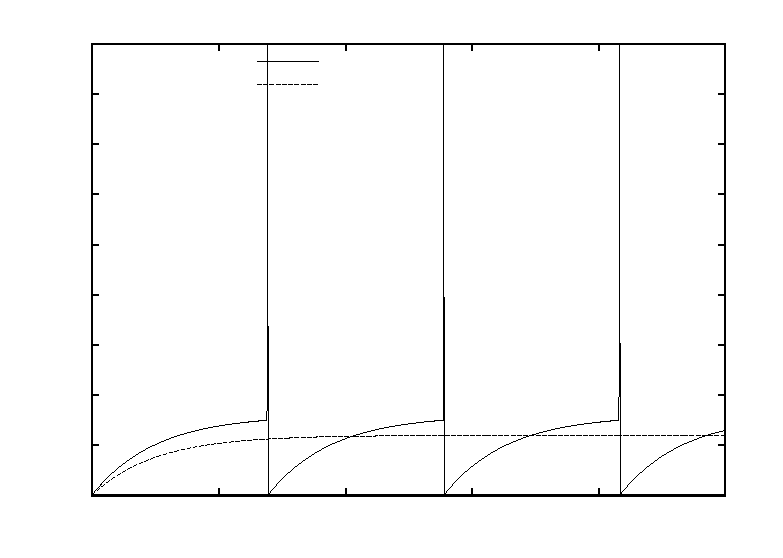
\includegraphics{v_i_f}}%
    \gplfronttext
  \end{picture}%
\endgroup

\end{center}
\caption{An integrate and fire neuron with different inputs. For
  $R_mI=12 $mV the voltage relaxes towards the equilibrium value
  $V=E_L+R_mI_e=-58$ mV. It never reaches the threshold value of
  $V_T=-55 $mV. For $R_mI=16$ mV the voltage reaches threshold and so
  there is a spike; the spike is added by hand, in this case by
  setting $V$ to $20$ mV for one time step. The voltage is then
  reset. Here $\tau_m=10$ ms.\label{v_i_f}}
\end{figure}

One thing to notice is that there are no spikes for low values of the current. Looking at the equation 
\begin{equation}
\tau_m\frac{dV}{dt}=E_L-V+R_mI_e
\end{equation}
so the equilibrium value for constant $I_e$, the value where $V$ stops changing, is
\begin{equation}
\bar{V}=E_L+R_mI_e
\end{equation}
Now if this value $\bar{V}>V_T$ then the neuron would spike before it
got there, if $\bar{V}<V_T$ then the neuron will not spike for that
input. We won't do it here, but, in fact, since we can solve the
equations for constant $I_e$ we can work out the $f-I$ curve, the
relationship between the firing rate and the input current. It is
plotted in Fig.~\ref{f_i_curve}.


\begin{figure}
\begin{center}
% GNUPLOT: LaTeX picture with Postscript
\begingroup
  \makeatletter
  \providecommand\color[2][]{%
    \GenericError{(gnuplot) \space\space\space\@spaces}{%
      Package color not loaded in conjunction with
      terminal option `colourtext'%
    }{See the gnuplot documentation for explanation.%
    }{Either use 'blacktext' in gnuplot or load the package
      color.sty in LaTeX.}%
    \renewcommand\color[2][]{}%
  }%
  \providecommand\includegraphics[2][]{%
    \GenericError{(gnuplot) \space\space\space\@spaces}{%
      Package graphicx or graphics not loaded%
    }{See the gnuplot documentation for explanation.%
    }{The gnuplot epslatex terminal needs graphicx.sty or graphics.sty.}%
    \renewcommand\includegraphics[2][]{}%
  }%
  \providecommand\rotatebox[2]{#2}%
  \@ifundefined{ifGPcolor}{%
    \newif\ifGPcolor
    \GPcolorfalse
  }{}%
  \@ifundefined{ifGPblacktext}{%
    \newif\ifGPblacktext
    \GPblacktexttrue
  }{}%
  % define a \g@addto@macro without @ in the name:
  \let\gplgaddtomacro\g@addto@macro
  % define empty templates for all commands taking text:
  \gdef\gplbacktext{}%
  \gdef\gplfronttext{}%
  \makeatother
  \ifGPblacktext
    % no textcolor at all
    \def\colorrgb#1{}%
    \def\colorgray#1{}%
  \else
    % gray or color?
    \ifGPcolor
      \def\colorrgb#1{\color[rgb]{#1}}%
      \def\colorgray#1{\color[gray]{#1}}%
      \expandafter\def\csname LTw\endcsname{\color{white}}%
      \expandafter\def\csname LTb\endcsname{\color{black}}%
      \expandafter\def\csname LTa\endcsname{\color{black}}%
      \expandafter\def\csname LT0\endcsname{\color[rgb]{1,0,0}}%
      \expandafter\def\csname LT1\endcsname{\color[rgb]{0,1,0}}%
      \expandafter\def\csname LT2\endcsname{\color[rgb]{0,0,1}}%
      \expandafter\def\csname LT3\endcsname{\color[rgb]{1,0,1}}%
      \expandafter\def\csname LT4\endcsname{\color[rgb]{0,1,1}}%
      \expandafter\def\csname LT5\endcsname{\color[rgb]{1,1,0}}%
      \expandafter\def\csname LT6\endcsname{\color[rgb]{0,0,0}}%
      \expandafter\def\csname LT7\endcsname{\color[rgb]{1,0.3,0}}%
      \expandafter\def\csname LT8\endcsname{\color[rgb]{0.5,0.5,0.5}}%
    \else
      % gray
      \def\colorrgb#1{\color{black}}%
      \def\colorgray#1{\color[gray]{#1}}%
      \expandafter\def\csname LTw\endcsname{\color{white}}%
      \expandafter\def\csname LTb\endcsname{\color{black}}%
      \expandafter\def\csname LTa\endcsname{\color{black}}%
      \expandafter\def\csname LT0\endcsname{\color{black}}%
      \expandafter\def\csname LT1\endcsname{\color{black}}%
      \expandafter\def\csname LT2\endcsname{\color{black}}%
      \expandafter\def\csname LT3\endcsname{\color{black}}%
      \expandafter\def\csname LT4\endcsname{\color{black}}%
      \expandafter\def\csname LT5\endcsname{\color{black}}%
      \expandafter\def\csname LT6\endcsname{\color{black}}%
      \expandafter\def\csname LT7\endcsname{\color{black}}%
      \expandafter\def\csname LT8\endcsname{\color{black}}%
    \fi
  \fi
  \setlength{\unitlength}{0.0500bp}%
  \begin{picture}(5040.00,3528.00)%
    \gplgaddtomacro\gplbacktext{%
      \csname LTb\endcsname%
      \put(814,704){\makebox(0,0)[r]{\strut{} 0}}%
      \put(814,1024){\makebox(0,0)[r]{\strut{} 10}}%
      \put(814,1344){\makebox(0,0)[r]{\strut{} 20}}%
      \put(814,1664){\makebox(0,0)[r]{\strut{} 30}}%
      \put(814,1984){\makebox(0,0)[r]{\strut{} 40}}%
      \put(814,2303){\makebox(0,0)[r]{\strut{} 50}}%
      \put(814,2623){\makebox(0,0)[r]{\strut{} 60}}%
      \put(814,2943){\makebox(0,0)[r]{\strut{} 70}}%
      \put(814,3263){\makebox(0,0)[r]{\strut{} 80}}%
      \put(946,484){\makebox(0,0){\strut{} 0}}%
      \put(1786,484){\makebox(0,0){\strut{} 5}}%
      \put(2626,484){\makebox(0,0){\strut{} 10}}%
      \put(3467,484){\makebox(0,0){\strut{} 15}}%
      \put(4307,484){\makebox(0,0){\strut{} 20}}%
      \put(176,1983){\rotatebox{-270}{\makebox(0,0){\strut{}firing rate in Hz}}}%
      \put(2794,154){\makebox(0,0){\strut{}$R_mI_e$}}%
    }%
    \gplgaddtomacro\gplfronttext{%
    }%
    \gplbacktext
    \put(0,0){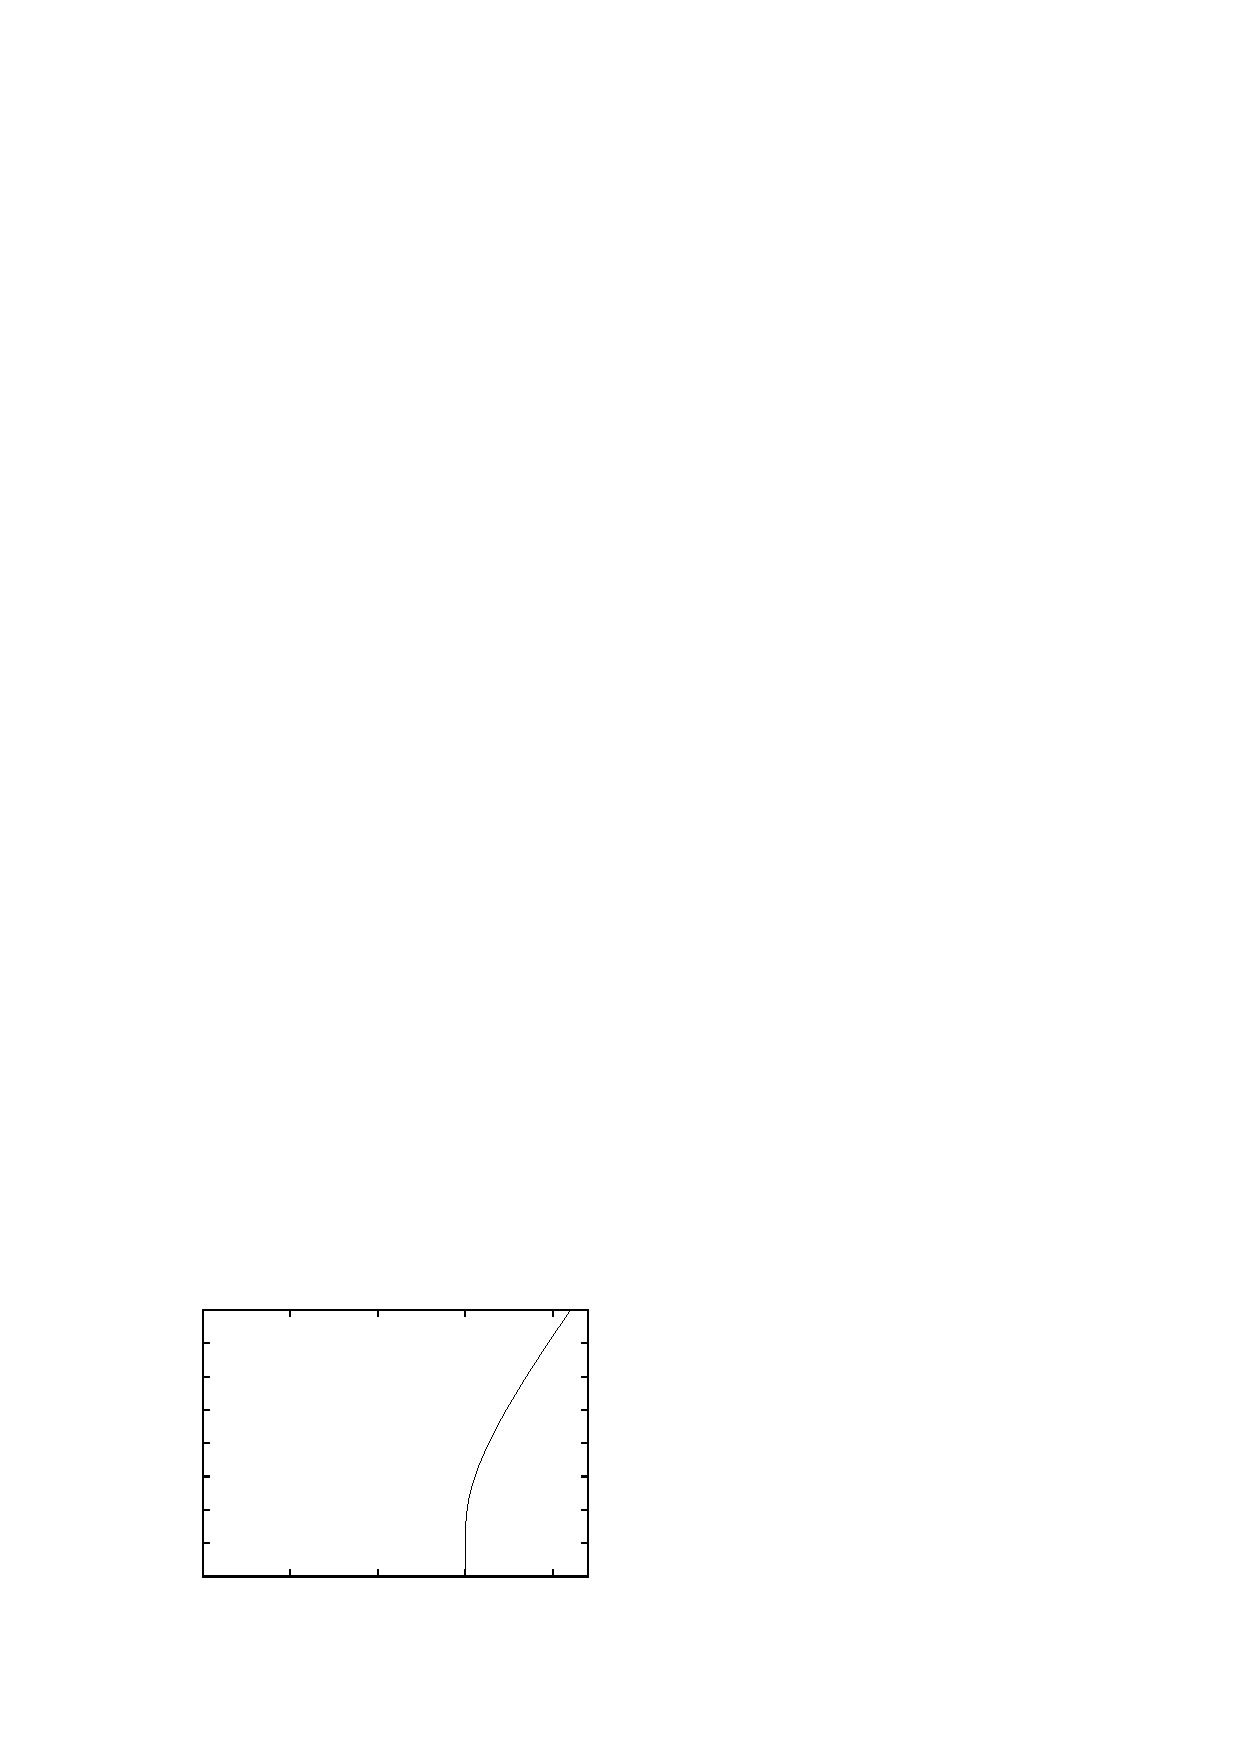
\includegraphics{f_i_curve}}%
    \gplfronttext
  \end{picture}%
\endgroup

\end{center}
\caption{The firing rate, that is spikes per second, for the integrate
  and fire neuron with different constant inputs with $\tau_m=10$ ms,
  $V_T=-55$ mV and both the leak and reset given by $-70$ mV. Notice
  how there is no firing until a threshold is reached and after that
  the firing increases very quickly. \label{f_i_curve}}
\end{figure}


\begin{thebibliography}{99}
\bibitem{Lapicque1907a}
Lapicque, L. (1907). 
\newblock Recherches quantitatives sur l'excitation �lectrique des nerfs trait�e comme une polarisation. 
\newblock J. Physiol. Pathol. Gen, 9:620--635.
\end{thebibliography}

\end{document}

